\texttt{minimum\_walk([0, 2, 3, 1], 0)}

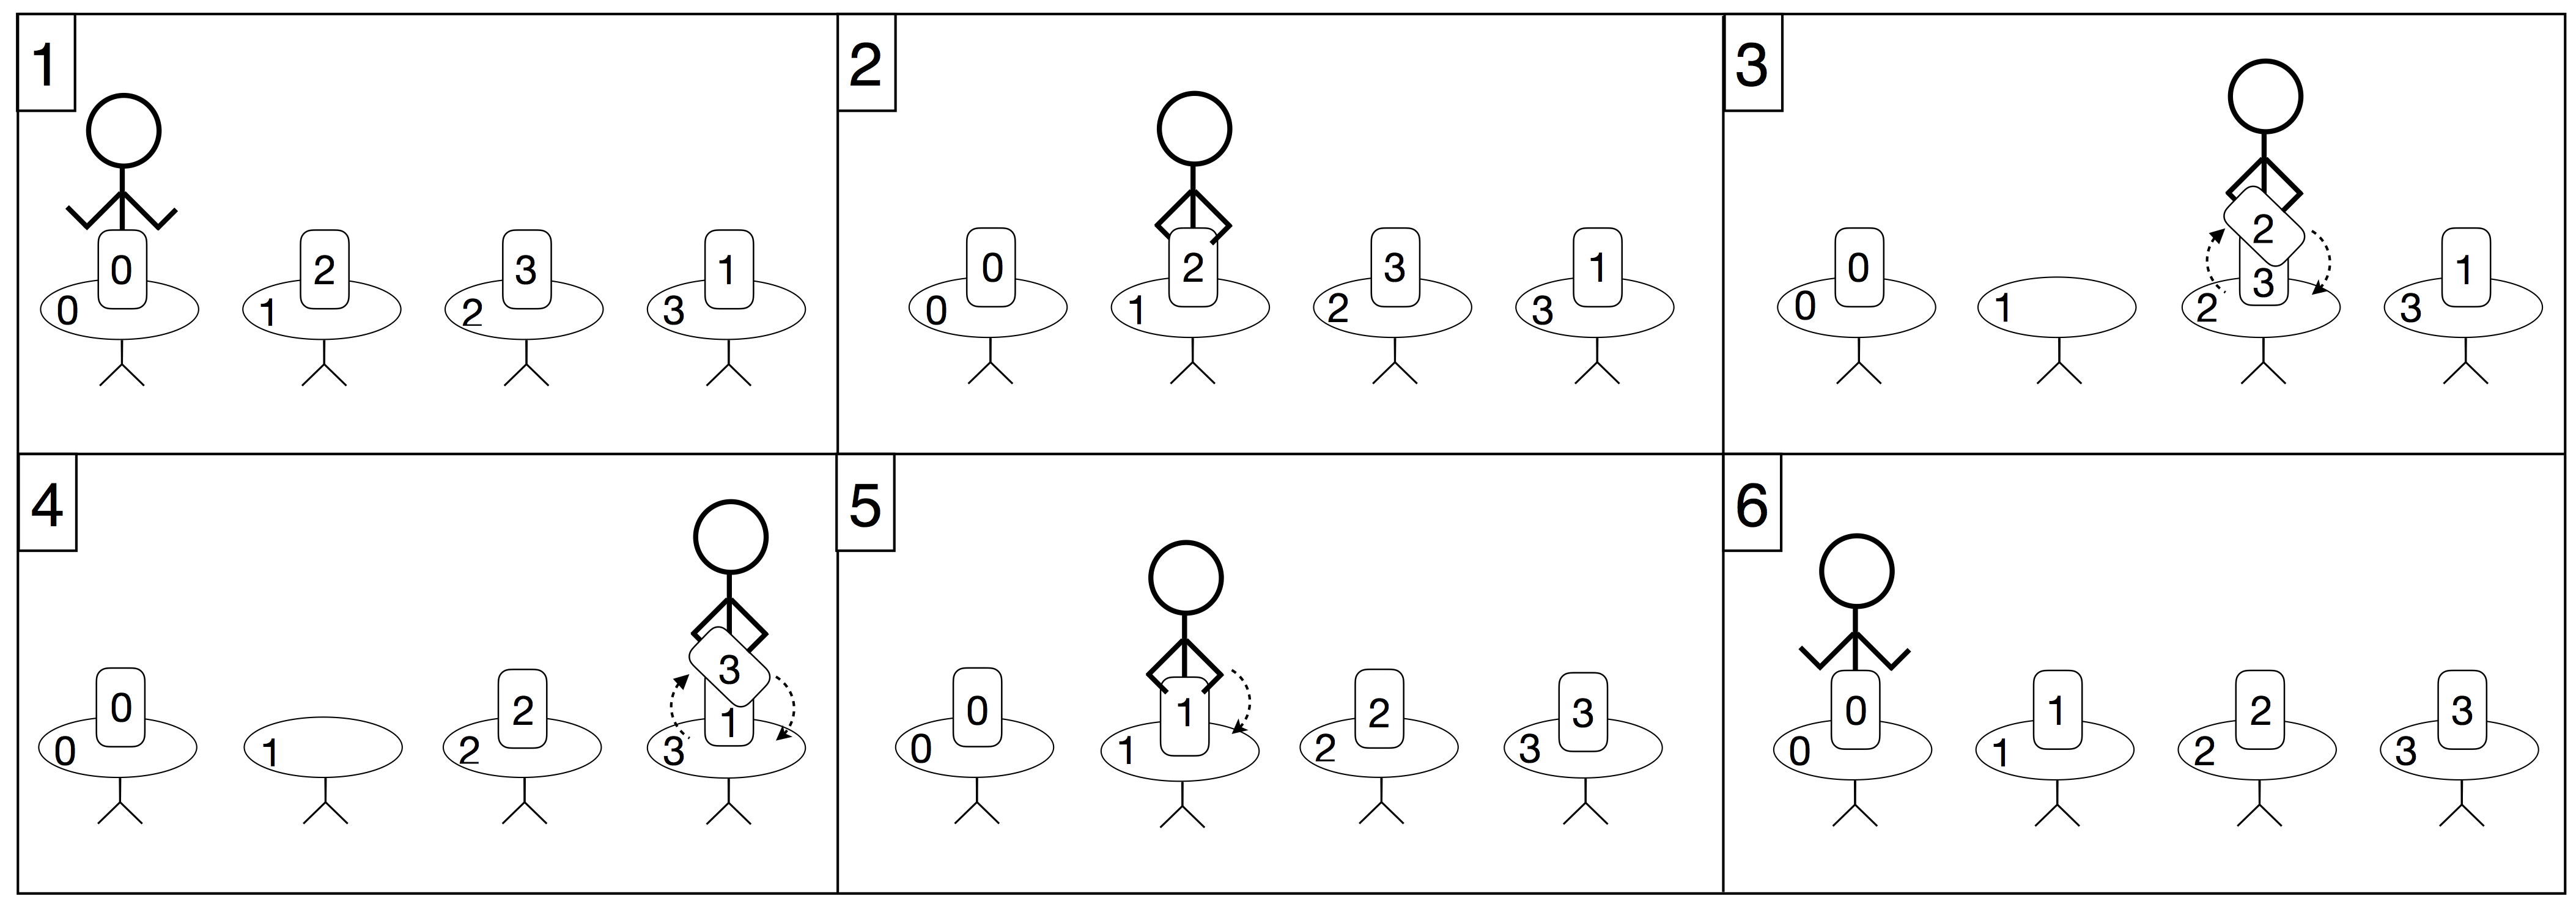
\includegraphics[scale=0.5]{books.png}

В этом примере $n = 4$, и Арьян начинает у стола $0$. Он может упорядочить книги следующим
образом:
\begin{itemize}
\item Подойти к столу $1$ и взять книгу с этого стола. Эту книгу необходимо положить на стол $2$.
\item Подойти к столу $2$ и поменять книгу, которую он держит, на книгу, лежащую на столе.
Книгу, взятую со стола, необходимо положить на стол $3$.
\item Подойти к столу $3$ и поменять книгу, которую он держит, на книгу, лежащую на столе.
Книгу, взятую со стола, необходимо положить на стол $1$.
\item Подойти к столу $1$ и положить на него книгу, которую он держит.
\item Наконец, вернуться к столу $0$.
\end{itemize}

Обратите внимание, что книга на столе $0$ уже находится на своем месте, поэтому Арьян не
обязан её переносить. Суммарное пройденное расстояние составляет $6$ метров. Этот способ
оптимален, поэтому функция должна вернуть $6$.